\chapter{Technical and Legal Background}

This chapter presents the technical foundations of browser extension development and the relevant European Union laws for compliance auditing. We provide a general overview here, while the detailed technical implementation of CookieAudit is discussed in \cref{ch:implementation}.

\section{Browser Extensions}
We implemented CookieAudit as a browser extension.
To understand the implementation details in \cref{ch:implementation}, we will give an overview about the architecture and implementation of browser extensions.

Browser extensions are programs that can extend and change the functionality of browsers.
They are built using web technologies (JavaScript, HTML, CSS) and can use APIs provided by the browser.
The APIs of Chromium based browsers (e.g., Chrome and Edge) overlap in large parts with the APIs of Mozilla's Firefox. Apple's Safari sometimes differs more significantly.
As a result, many extensions can run in several browser environments.

When building browser extensions, developers have to split up their code in a predefined (as specified by Manifest Version 3~\cite{manifestv3} for Chromium based browsers).
We will first explain the different parts of a general browser extension architecture and detail the challenges posed by Manifest V3 in \cref{subsec:manifest-v3}.
A visualization of the building blocks and their interactions is shown in \cref{fig:extension-architecture}.

\begin{figure}
	\centering
	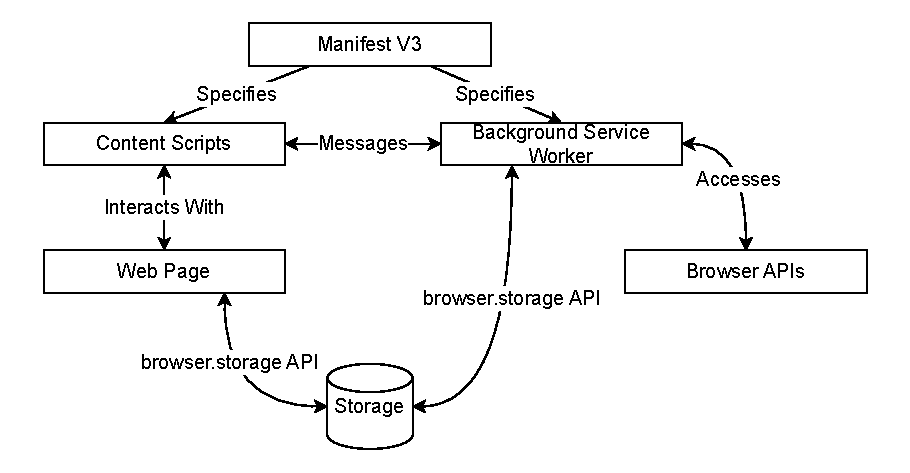
\includegraphics[width=\textwidth]{media/browser-extension-architecture.drawio.pdf}
    \caption{The general architecture of a manifest version 3 browser extension.}
    \label{fig:extension-architecture}
\end{figure}

\subsection{Extension Service Workers} \label{subsec:service-workers}
The Extension Service Worker is the central location for business logic.
By having access to the full WebExtensions API, it is the place to define event listeners\footnote{
By registering event listeners at the beginning of the service worker, developers can define code that is to be run on browser, tab or extension events to handle e.g., extension messages or the user visiting a different URL.},
send and receive messages to and from the extension building blocks 
or run time intensive computations~\cite[Ch. 4]{frisbie2023browser}.
Service workers operate asynchronously on a separate thread, preventing interference with website execution. 
They are ephemeral, terminating when idle and restarting to handle events. Developers must persist important application state to storage (see \cref{subsec:storage}) rather than relying on in-memory variables, as these are reset upon termination.

\subsection{Content Scripts} \label{subsec:content-scripts}
Content scripts are JavaScript programs injected into web pages. 
They can access and modify the page's HTML structure and CSS styles.
By default\footnote{
Developers can deactivate this isolation by setting the execution world to \texttt{MAIN}. Then, the content script will be able to e.g., read variables of the web page JavaScript.
}, content scripts run in an isolated environment, separate from the page's own JavaScript.
This isolation prevents direct access between the content script and page script.
Variables are not shared, and functions from one context cannot be called by the other.
Content scripts have limited access to WebExtensions API. 
For example, they cannot change the current tab's URL.
To interact with the rest of the extension, content scripts use messaging and a shared key-value store (see \cref{subsec:storage}).

\subsection{Communication}
From the perspective of the developer, the extension service worker and the different content scripts run in separate environments. 
As a result variables and functions cannot be accessed across those boundaries.
Instead, browsers provide the messaging API to send and listen for messages (example in \cref{fig:message-passing}).

\begin{figure}
	\centering
	\definecolor{backcolour}{rgb}{0.95,0.95,0.92}
	\lstset{backgroundcolor=\color{backcolour}}
	    
	\begin{subfigure}{\textwidth}
		\centering
		\begin{lstlisting}
let response = await chrome.runtime.sendMessage({
  cookieNoticeDetected: true
});
		\end{lstlisting}
		\caption{Sending a message from the content script}
	\end{subfigure}
	    
	\begin{subfigure}{\textwidth}
		\centering
		\begin{lstlisting}
function handleMsg(request,sender,sendResponse) {
  // ... handle message inside request object ...
  // send response to content script:
  sendResponse({ storedData: true });
}
chrome.runtime.onMessage.addListener(handleMsg);
		\end{lstlisting}
		\caption{Handling a message in the background script}
	\end{subfigure}
	    
	\caption{Message passing in Chrome extension}
	\label{fig:message-passing}
\end{figure}

\subsection{Storage} \label{subsec:storage}
Browser extensions often need to be able to store data, even across browser restarts.
Developers can therefore use the asynchronous\footnote{Even though JavaScript is single-threaded, its asynchronous mechanisms allow non-blocking execution, handling tasks like I/O operations without halting the main thread.} storage API to store key-value pairs serialized as JSON objects. Serializable types include primitives, Arrays, and Objects, but not Functions or \verb|HTMLElement|.

\subsection{Manifest Version 3} \label{subsec:manifest-v3}
We have developed CookieAudit according to Manifest version 3~\cite{manifestv3}.
It is the newest specification of the extensions API for Chromium based browsers.
Compared to Manifest version 2, it includes API changes and restrictions aimed to increase the security and performance of extensions.
Version 3 has forced some developers to make considerable changes to their extensions.
We will present the some breaking changes between Manifest version 2 and 3.

\subsubsection{Background Scripts to Service Workers}
In Manifest version 2 developers could use \verb|background scripts| which effectively were non-visible, persistent web pages.
Many extensions developed for manifest version 2 used the fact that background scripts are never terminated and global variables of the background script are accessible from the popup.
As explained in \cref{subsec:service-workers}, developers cannot rely on those characteristics anymore.
The migration to manifest version 3 sometimes required considerable changes in the architecture of extensions\footnote{
The switch to service workers in the Bitwarden password manager greatly increased complexity~\cite{gonzalez2024bitwarden}}.

\subsubsection{Execution of Arbitrary Strings}
The execution of arbitrary strings with the \verb|eval()| function can be used for security exploits as shown by Carlini et al.~\cite{carlini2012evaluation}.
To solve this issue, it is no longer possible to evaluate and execute strings using methods such as \verb|eval()|, or \verb|new Function()|.
It is still possible to evaluate and execute WebAssembly\footnote{WebAssembly is an assembly language that can be compiled to from languages like C++ or Rust. It provides high performance but also easy interfacing between JavaScript and WebAssembly functions~\cite{a2024webassembly}.}, by specifying \verb|wasm-unsafe-eval| in the extension manifest.
This is necessary for many performance critical applications, such as the client-side inference of AI models.

Other breaking changes introduced in Manifest version 3 are 
\begin{itemize}
    \item limitations to the inspection and modification of live requests
    \item no more execution of remotely hosted code
    \item renaming and restructuring of certain WebExtensions API functions
\end{itemize}



\section{General Data Protection Regulation and ePrivacy Directive} \label{sec:legal}
Both the General Data Protection Regulation (GDPR)~\cite{gdpr2016} and ePrivacy Directive~\cite{privacydirective2016} have regulated the processing of personal information for entities targeting people inside the European Union.
The GDPR generally requires a legal basis defined in Article 6 for the processing of personally identifiable information such as names, identification numbers or location data.
If an entity such as a company wants to use the data for analytics or advertising, the user has to provide consent that is "freely given, specific, informed and unambiguous indication of the data subject's agreement to the processing of personal data relating to him or her" (Recital 32 GDPR).
The 2002 ePrivacy Directive similarly requires consent for the usage of technologies like cookies, except in cases where they are necessary\footnote{An example of a functionally required cookie would be a token to let the user stay signed into his account across browser sessions.} for the functionality of a website.